%___________________________________________________________________________________________________
\chapter{Operations with vectors and matrices}    \label{chap:matrices}


\vspace{-.7cm}
\section{Introduction}

This chapter covers two independent topics through examples. 
In the first place, some essential operations of matrix arithmetic are introduced, 
an operation like the product of two matrices becomes extremely simple 
in programming languages oriented to vector programming. 
In the second place, the concepts of static and dynamic data objects are covered. 
Notice that all the examples are written according to a declarative programming style, 
consider reproducing the same results with an imperative programming style to compare.
    
    \vspace{-.3cm}
    \subsection*{Matrix arithmetic}
    \vspace{-.2cm}

An array programming language or vector language has the possibility 
to operate a whole group of values at once.
The common operations that range over scalar numbers can then be applied to vectors, 
matrices and higher dimension arrays in a closer to maths style. 
Hence, mathematical expressions at the time of programming are simplified.

Languages like Fortran, MATLAB, R or the NumPy extension of Python support array programming.
Matrix arithmetic are built-in in these languages and expressing the mathematical language in a natural way is feasible.

\newpage
The following concepts are covered:
\begin{enumerate}[noitemsep]
    \item Declaring arrays (Fortran): type, rank and dimension.
    \item Initialize arrays: constructors. 
    \item Iterators for arrays, sectors or slices. 
    \item Operations:
    \begin{itemize}
        \item Addition. 
        \item Dot product.
        \item Matrix multiplications. 
        \item Hadamard product. 
        \item Element-wise operations.    
    \end{itemize}
\end{enumerate}  


%Take note of the difference between array programming and array processors. The first makes reference to how the programmer 
%codes the mathematical operations in its program (a big advantage is obtained from this feature for Scientific Computing as mentioned before). 
%The second feature is related to how the processor operates that group of numbers, by performing
%all the operations together under the same instruction given to the processor in a considerably increase of speed.
%Both features suppose an increase of performance for the coding and executing of scientific programs, however, this chapter is 
%oriented to the aspects of the first feature mentioned. 



    \vspace{-.5cm}
    \subsection*{Static/Dynamic data objects}

Each data object declared in a program (variables, constants, pointers, arrays, etc.) are either static or dynamic, 
this means that the memory storage to hold that piece of data is reserved during compilation time or 
during the execution of the program respectively. 

Consider for example the Fortran variable \texttt{real :: A(N, N)} declared at the beginning of a code, 
its memory storage is reserved when the program is compiled and this space is not liberated 
until the program has finished the execution. 

Another option to declare and manage the memory storage of an object involves using dynamic allocation. 
In this case, the storage of the variable is not reserved until the program orders it (which happens during the execution of the code) and can be changed or freed at any moment. 
In Fortran for example, this is done through a code like \texttt{real, allocatable :: Ak(:, :, :)}.

This chapter also includes a review of the main memories that a program uses: Static, Heap and Stack.
All variables, program instructions, constants, etc. are stored in these memories and their use is intimately related 
to the different ways of allocating space in the code.





%___________________________________________________________________________________________________
\newpage 
\section{Declaring, initializing and slicing arrays} 
%Declaration
Consider the vectors $V \in \mathbb{R}^N$, $X\in \mathbb{R}^6$, $Y\in \mathbb{R}^3$ 
and matrices $A \in { \cal{M}}^{N \times N} (\mathbb{R})$, $Z \in { \cal{M}}^{2 \times 3} (\mathbb{R})$
with $N=10$ and let's use arrays to represent them: 
$$
V = \left( v_i =\frac{1}{i^2} \right)^T, \quad A = \left[ a_{ij} = \left( \frac{i}{N} \right)^{j-1} \right], \;\; i = 1 \ldots  N, \;\;  j = 1 \ldots  N   
$$
$$
X = ( 1.3, 2.4, 3, 4.5, 5.3, 7 )^T,  \quad  Y = \left(A_{i j}\right)_{\substack{i = 2 \\  3\leq j\leq 5}}^T, \quad Z =     
\begin{bmatrix}
    1.1 & 2.2 & 3.3\\
    4 & 5.6 & 6.2
\end{bmatrix} 
$$

    \subsection*{Fortran code}

An array, either representing a vector, a matrix or a tensor, is properly \textbf{declared} when it has 
type, rank and dimension (or extent) (see Figure \ref{fig:arrays}). 
The data type has already been treated before, in these examples we are using \texttt{real} vectors and matrices. 
The rank; the number of dimensions in the array, is 1 for column vectors, 2 for matrices and can be higher for higher dimension tensors.
The extent of each particular dimension is its length; the number of elements in that dimension.
\vspace{0.5cm}
\lstfor
\renewcommand{\home}{./Fortran/sources/Foundations/Algebra} 
\listings{\home/Matrix_operations.f90}{subroutine Basic_arrays}{indices of B}{Basic_operations.f90}

\begin{IN}
    Notice that, in Fortran, the \textbf{bounds of a dimension} may start with the index we prefer. 
    By default it stars with index \texttt{1} but it can start in \texttt{0} or whatever index we want. 
    For example the matrix \texttt{B(-2:4,0:1)} starts in \texttt{-2} and ends in \texttt{4} (also included) for the first dimension and 
    \texttt{0} and \texttt{1} (also included) for the second dimension. 
\end{IN}


\newpage
%Initialization
Once declared, the \textbf{initialization} of the arrays is performed with constructors. 
Three ways are commonly used to manually construct an array: 
\vspace{-0.5cm}
\begin{enumerate}[noitemsep]
    \item \textbf{List of values:} \texttt{ [ list ] } where 'list' is a list of values of the same array type separated by commas. 
    \item \textbf{Array slice:} For example \texttt{Y = [ A(2, 3:5) ]} stores the list of values in the second row of \texttt{A} from columns \texttt{3} to \texttt{5}.
    \item \textbf{Implicit loop:} a list of elements is computed from a loop.
\end{enumerate}
In Fortran a list of values can only be used with rank-one arrays so 
the function \texttt{reshape} is needed for higher ranks. 
For example the matrix \texttt{A} in the code is initialized using the \texttt{reshape} function.     
\vspace{0.5cm}
\lstfor
\renewcommand{\home}{./Fortran/sources/Foundations/Algebra} 
\listings{\home/Matrix_operations.f90}{Implicit loop}{By columns}{Basic_operations.f90}   




%sectors, iterators... 
In Fortran the elements of the array are accessed using parenthesis notation and
an index in each dimension can be used as \textbf{iterator}.
This is intimately related to the \textbf{slicing}: referencing a portion of the array by a range of indices.
For example the initialization of \texttt{Y} above use an slice of \texttt{A}.
This can also be extended to a whole dimension using the colon symbol, \texttt{C(:,2)}. 
Furthermore, alternate values can be selected by specifying a lower bound, an upper bound and the jump between values.
Notice that, since Fortran is a column major order language, functions like \texttt{reshape} and slicing treats the data by columns. 
\vspace{0.5cm}
\lstfor
\renewcommand{\home}{./Fortran/sources/Foundations/Algebra} 
\listings{\home/Matrix_operations.f90}{Slices}{columns!}{Basic_operations.f90}  




    \newpage
    \subsection*{Python code}

Let's see the same examples defined above using \texttt{NumPy} arrays.
Notice that now they do not need to be explicitly declared, 
Python automatically does it. 

%Initialization
The \textbf{initialization} of the arrays is performed using the \texttt{array()} function as constructor. 
Three ways are commonly used to manually construct an array: 
\begin{enumerate}[noitemsep]
    \item \textbf{List of values:} \texttt{ [ list ] } or \texttt{ [ [ list ], [ list ] ] } for higher than rank-one arrays,
     where \texttt{list} is a list of values of the same array type separated by commas.
    \item \textbf{Array slicing:} For example \texttt{Y = A(1, 2:5)} stores the list of values in the second row of \texttt{A} from columns \texttt{3} to \texttt{5}.
    \item \textbf{Implicit loop (list comprehension):} a list of elements is computed from a loop.
\end{enumerate}
\vspace{0.5cm} 
\lstpython
\renewcommand{\home}{./Python/sources/Foundations/Algebra} 
\listingsp{\home/Matrix_operations.py}{basic_arrays}{by rows}{data_type.py}



%sectors, iterators...    
In Python, the elements of the array are accessed using bracket notation, 
the array can be \textbf{iterated} using an index in each dimension and 
\textbf{slicing} is also allowed.
Notice that NumPy arrays, contrary to Fortran, are row-major order. 
This means that arrays store the data by rows. 
Similarly to Fortran, the colon symbol iterates in a whole dimension and 
alternate values can be selected by specifying lower and upper bound and the jump between values.
However, the example \texttt{B(-2:4:3,:)} made with Fortran can not be copied because:
\begin{IN}
    In Python, the \textbf{bounds of a dimension} always start with the index \texttt{0} (zero-indexing) and
    stop 1 before the final bound.  
\end{IN}



\newpage
%\begin{figure}[h]
%    \centering
%    \includegraphics[width= 0.8\textwidth]{./doc/Figures/FixedFloat3.png}
%    \caption{Representation of number 20.25 with fixed-point format using only 1 byte (8 bits).}
%    \label{fig:FixedFloat2}
%\end{figure}
\FloatBarrier
\begin{figure}[b]
    \centering
    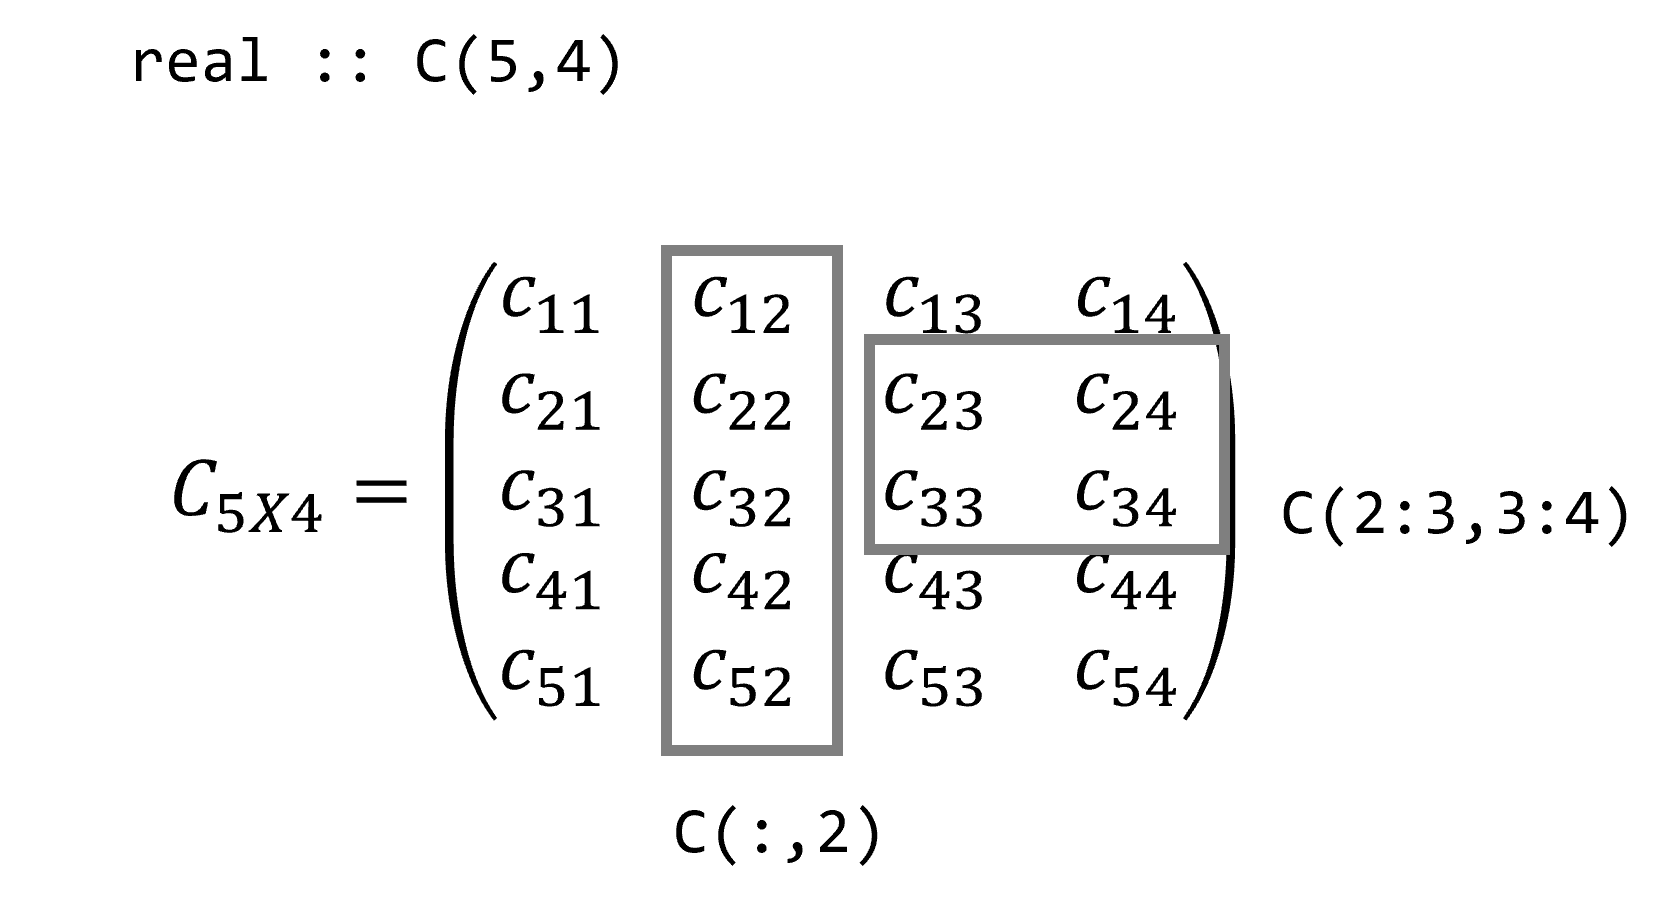
\includegraphics[width = .8\textwidth]{./doc/Figures/Array1.png}  \\
    \begin{center}
        Rank = 2 \\
        Extent = (5,4) \\
        Size = 20 \\
        Bounds = (1:5, 1:4) \\
        %Shape = (5, 4)
    \end{center}
\end{figure}

\begin{figure}[b]
    \centering
    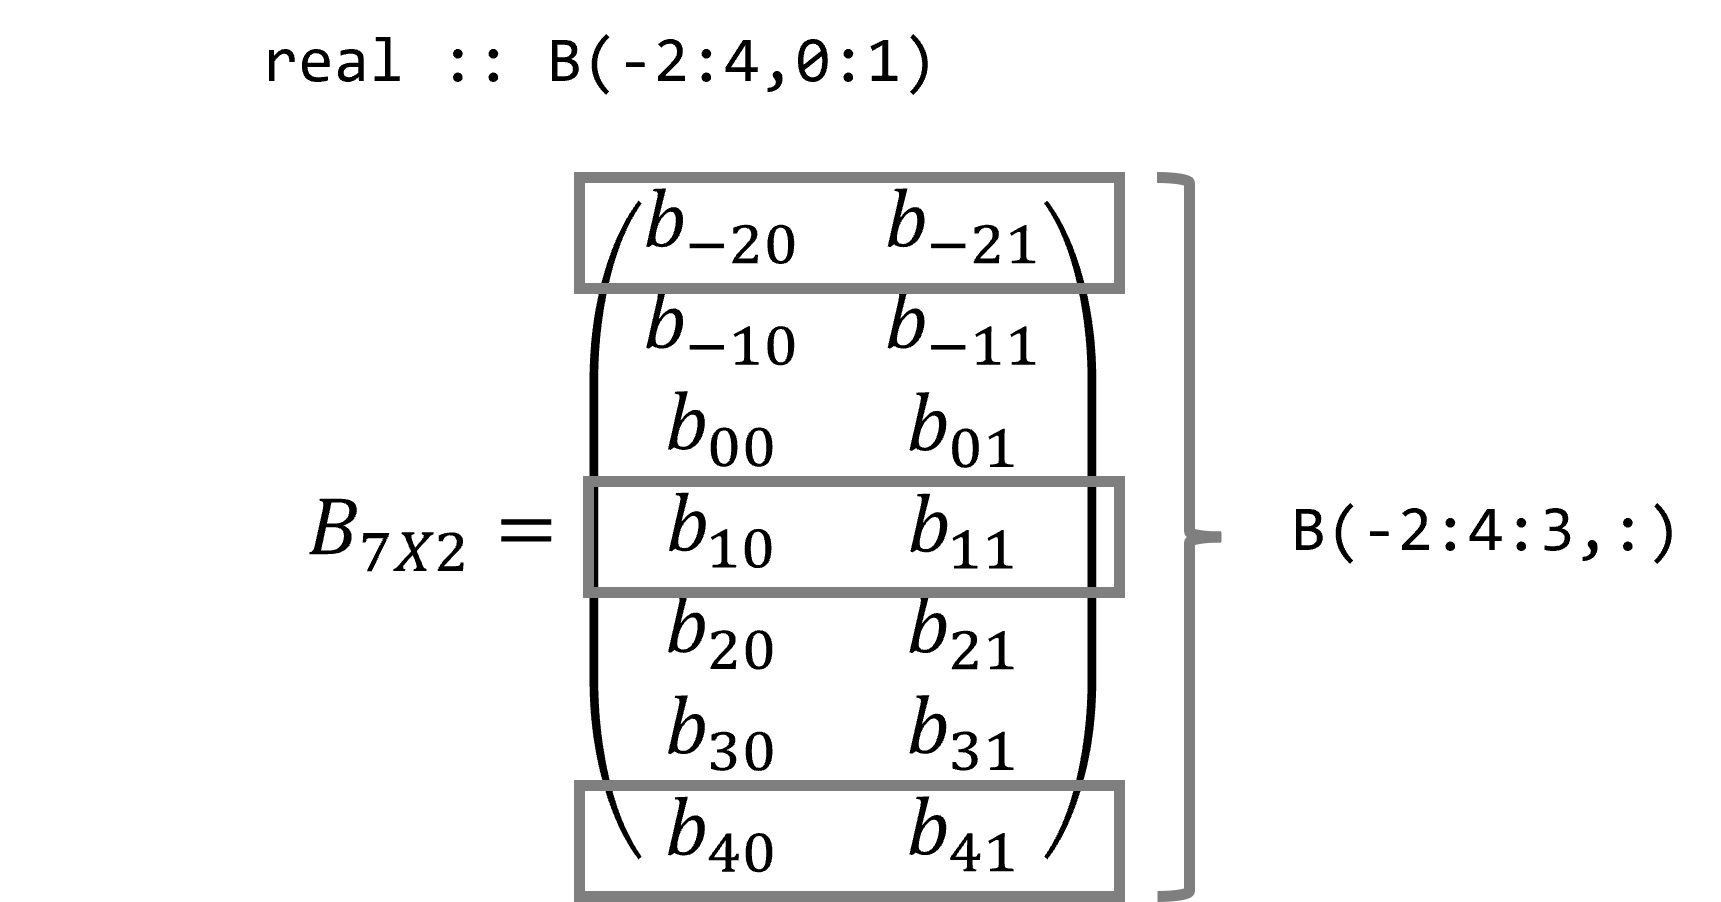
\includegraphics[width = .8\textwidth]{./doc/Figures/Array3.png}  \\
    \begin{center}
        Rank = 2 \\
        Extent = (7,2) \\
        Size = 14 \\
        Bounds = (-2:4, 0:1) \\
        %Shape = (7, 2)
    \end{center}
\caption{Example arrays with their main properties.}   \label{fig:arrays}
\end{figure}

%\begin{figure}
%    \begin{subfigure}[b]{0.5\textwidth}
%        \centering
%        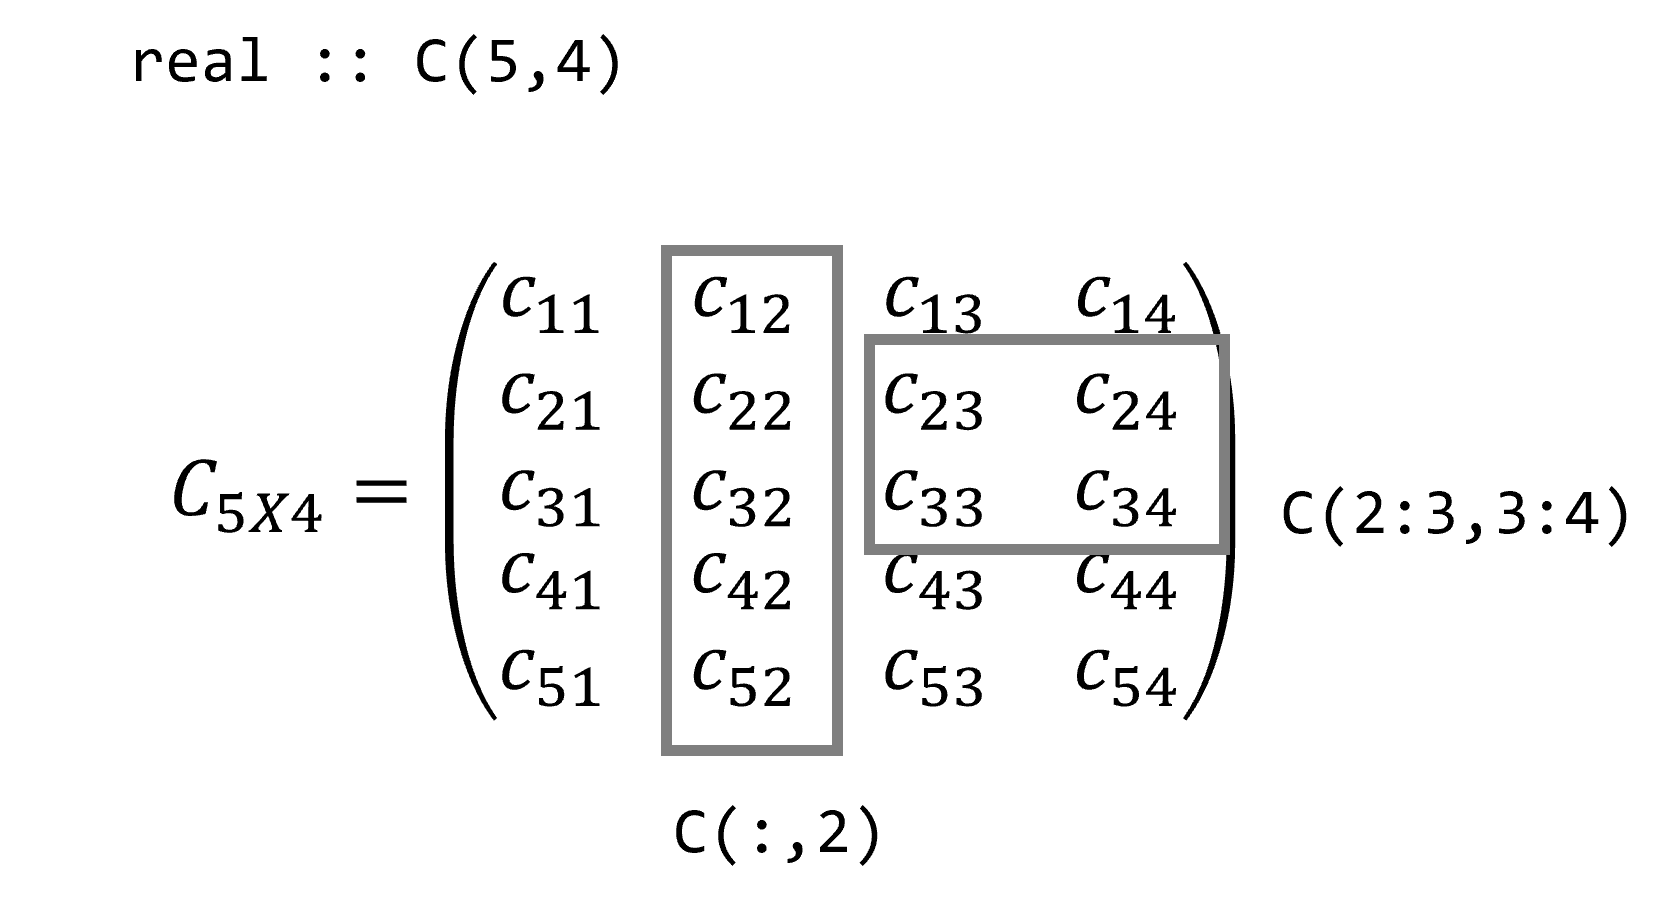
\includegraphics[width = \textwidth]{./doc/Figures/Array1.png}  \\
%        \begin{center}
%            Rank = 2 \\
%            Extent = (5,4) \\
%            Size = 20 \\
%            Bounds = (1:5, 1:4) \\
%            %Shape = (5, 4)
%        \end{center}
%    \end{subfigure}
%    \hspace{\fill}
%    \begin{subfigure}[b]{0.5\textwidth}
%        \centering
%        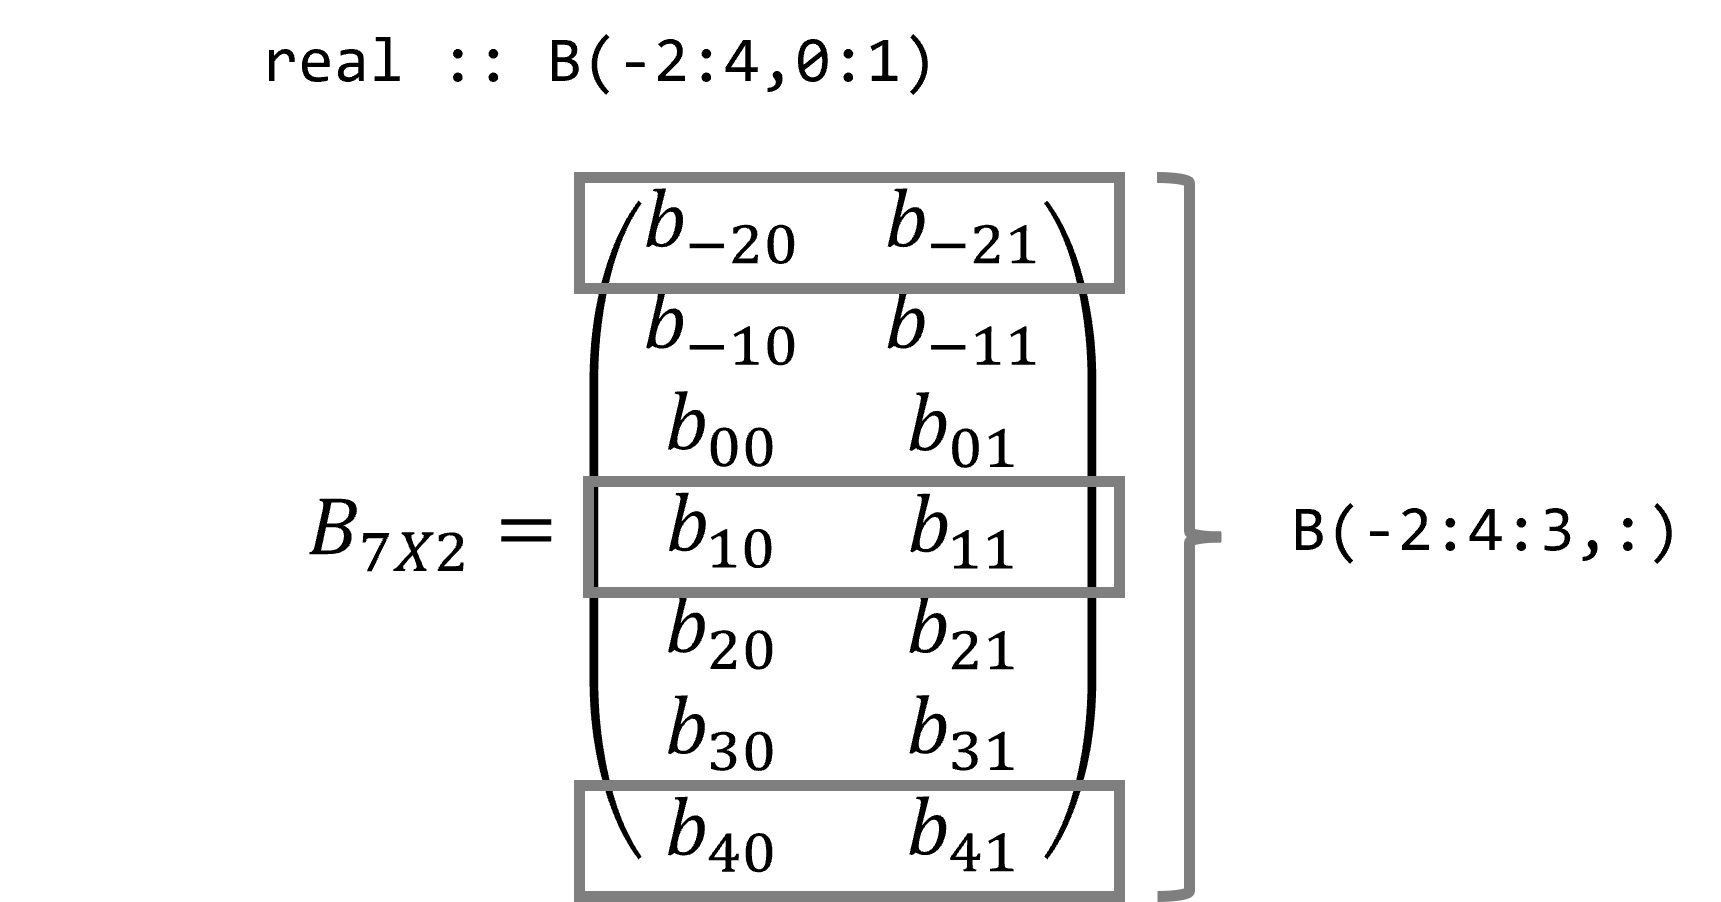
\includegraphics[width = \textwidth]{./doc/Figures/Array3.png}  \\
%        \begin{center}
%            Rank = 2 \\
%            Extent = (7,2) \\
%            Size = 14 \\
%            Bounds = (-2:4, 0:1) \\
%            %Shape = (7, 2)
%        \end{center}
%    \end{subfigure}
%    \caption{Example arrays with their main properties.}   \label{fig:arrays}
%\end{figure}


\FloatBarrier


%___________________________________________________________________________________________________
\newpage 
\section{Static size vectors and matrices} 

Consider the same vectors $V, W \in \mathbb{R}^N$ and matrices $A, B \in { \cal{M}}_{N \times N} (\mathbb{R})$ used in the previous section (with $N=10$): 
$$
V = \left[ v_i =\frac{1}{i^2}, \ \ i = 1 \ldots  N \right],
$$
$$
W = \left[ w_i = \frac{(-1)^{i+1}}{2i+1}, \ \ i = 1 \ldots  N \right],
$$
$$
A = \left[ a_{ij} = \left( \frac{i}{N} \right)^{j-1}, \ \ i = 1 \ldots  N, \ \ j = 1 \ldots  N \right],
$$
$$
B = A^T
$$
and let's compute the following matrix operations:
$$
1.\;\sum_{i=1}^N v_i  \qquad \qquad 2.\;\sum_{i,j=1}^N a_{ij}   \qquad \qquad   3.\;\sum_{v_i>0} v_i   \qquad \qquad 4.\;\sum_{\scriptstyle i,j=1 \atop \scriptstyle a_{ij} > 0.1}^N a_{ij}   
$$
$$
5.\; V\cdot W^T    \quad \quad      6.\; V\cdot [a_{ij}]_{\scriptstyle 1\leq i\leq N \atop \scriptstyle j = N}    \quad  \quad  7.\; AV     \quad \quad   8.\;\sum_{i,j=1}^N [A^2]_{ij}   \quad \quad    9.\; B = A^T
$$
$$
10.\;\max_{1\leq i,j\leq N} \{ a_{ij} \}       \qquad \qquad     11.\;\arg\max_{1\leq i,j\leq N} \{ a_{ij} \}   
$$

Apart from matrix operations, programming languages also support element-wise operations,
those where the result is an equal shaped array with the results of applying the operation to each/corresponding elements.
Let's compute for example the addition of two matrices, the Hadamard product (where corresponding elements are multiplied)
or some elemental operations that can also be applied to matrices apart from numbers: cosine or square root. 
Notice that, where needed $i,j = 1\ldots N$ with $N=10$:
$$
1.\;\Tr(A + B)  \quad \quad 2.\;\Tr(A\odot B)  \quad \quad   3.\;\Tr( \left[ cos( a_{ij} )\right] )   \quad \quad 4.\;\Tr( \left[ \sqrt{a_{ij}} \right] )
$$

Since the sizes of these arrays are known at compile-time, the memory storage can be declared statically. 
The main properties of a static allocation are:
\begin{enumerate}
    \item The memory address and the size are assigned during the compilation of the code in the executable image of the program.
    \item These address and size can not be changed during execution.
    \item Once the program finishes the execution the space is freed.
    \item It is a simple and quick allocation process.
\end{enumerate}



        \newpage
        \subsection*{Fortran code}
The following code computes these operations using Fortran. 
Notice that these examples are limited to numeric arrays: integers, reals or complex,
however, arrays can be constructed with a different data type. 
Furthermore, new operations could be defined for other data types. 
    
Consult the specifications of the following matrix operations to become familiarized with the purpose, inputs and arguments.
Notice that the rank and dimension of the arguments must agree with the mathematical definitions of the operations.
As a quick reference: 
\begin{itemize}[noitemsep]
    \item \texttt{sum} adds all elements of an array: across one dimension, all the dimensions 
    or only the elements that accomplish with some condition (e.g. $v_i > 0$).
    \item \texttt{dot\_product} calculates the scalar product of two vectors.
    \item \texttt{matmul} computes a matrix multiplication. 
    \item \texttt{transpose} calculates the transpose of a matrix or vector. 
    \item \texttt{maxval} and \texttt{maxloc} return the maximum value from all the elements of an array and its position respectively.
    It can compute the result across one dimension, the whole array or only for those values that accomplish with a specified condition.
\end{itemize}

\lstfor
\renewcommand{\home}{./Fortran/sources/Foundations/Algebra} 
\listings{\home/Matrix_operations.f90}{subroutine Matrix_operation_examples}
      {end subroutine}{Matrix_operations.f90}

Let's remark some interesting notes of this code. 
First of all, \texttt{N} (which declares the size of the arrays) is declared as a named constant thanks to the \texttt{parameter} attribute. 
Hence, its value is fixed during the whole execution and a try to change it returns a compilation error. 

Secondly, to initialize both \texttt{V} and \texttt{W} their definition is written by means of an implicit loop (declared with parentheses). 
To define the matrix \texttt{A} two implicit loops are used: 
the nested loop \texttt{i} iterates in the rows while 
\texttt{j} jumps from one column to the next one. 
Both loops define a $N\cdot N$ rank-one vector that needs to be reshaped to a ${\mathbb{R}}^{N\times N}$ matrix. 
The function \texttt{reshape} organizes the components of the vector into columns. 

Finally, notice how an implicit loop with a colon symbol \texttt{:} is also used
in the scalar product of the vector \texttt{V} with the $N$-th column of \texttt{A}. 
The implicit loop in \texttt{A} iterates in the \texttt{N} elements of the column. 
Another example would be how the matrix \texttt{B} is written in the screen,
it uses two loops (one explicit and one implicit) so each row of the matrix is represented element by element.
Compare this way with the output of the line \texttt{write(*,*) B} where all the elements are represented by columns and not by rows. 
This is due to the fact multidimensional arrays are stored in a linear storage and Fortran,
which is a \textit{column-major order} language, organizes the consecutive elements of a column one next to each other.

The following code computes the proposed element-wise operations using Fortran.
\vspace{0.5cm} 
\lstfor 
\listings{\home/Matrix_operations.f90}{subroutine ElementWise_operation_examples}
{end subroutine}{Matrix_operations.f90}




         \newpage 
        \subsection*{Python code}
The same function can be written almost identically with Python. 
Notice from the following code how all vectors and matrices are constructed by using similar implicit loops. 
In addition, the same intrinsic functions are implemented so the use of mathematical notation when programming becomes natural.
Some particularities in this examples would be the indentation or the use of implicit typing. 
%\vspace{0.5cm} 
\renewcommand{\home}{./Python/sources/Foundations/Algebra} 
\lstpython
\listingsp{\home/Matrix_operations.py}{def Matrix_operation_examples}
      {WARNING}{Matrix_operations.py} 

The following code computes the proposed element-wise operations using Python.
\vspace{-.5cm}
\lstpython
\listingsp{\home/Matrix_operations.py}{def ElementWise_operation_examples}
{END}{Matrix_operations.py}





%_______________________________________________________________________________________________
\newpage  
\section{Dynamic allocation of vectors and matrices} 

Now let's use the square Vandermonde matrix  of $M\times M$:
$$
A_M =  \left[ a_{ M_{ij} } = \left( \frac{i}{M} \right)^{j-1}, \ \ i = 0, \ldots M-1, \ \  j=0, \ldots M-1 \right],  
$$
to compute the following operations:
$$ 
S = \sum_{M=1} ^{10} \Tr(A_M)  \qquad
S = \sum_{M=1} ^{5} \Tr(A_M^2) \qquad
S = \Tr \left( \sum_{k=0} ^{5} A_M^k  \right)  \qquad  M=8 
$$

Imagine now that the size of the matrix involved in your code is not known at compile-time, maybe it comes from 
an user input, 
an external file or 
it is the result of a previous operation. 
In this case, dynamic data objects are used so its memory storage (address, size, etc.) is allocated or modified during the execution of the program.
In Fortran for example the essential statements used to manage the memory are 
\texttt{allocate} and \texttt{deallocate} while the attribute for the data object is \texttt{allocatable}. 
The main properties of dynamic data objects are:

\begin{enumerate}
    \item The program decides how much memory reserve for a data objects so it can accommodate any size with no need of re-compiling the code.
    \item Modifications for the memory size are allowed. 
    \item It becomes the programmer responsibility to liberate the memory reserved for non-used arrays in order not to run out-of-memory.
    \item It is generally slower than static allocation. 
\end{enumerate}

The following examples, whether coded in Fortran or Python, are based on the following functions: 
\begin{itemize}[noitemsep]
    \item \texttt{Vandermonde( M )} which computes the Vandermonde matrix of a given dimension \texttt{M},
    \item \texttt{trace( A )} to compute the trace of a matrix and
    \item \texttt{power( a, k )}, a recursive function to obtain the $k$-th power of a matrix.
\end{itemize}
Once each function is coded, more general operations are easy to implement. 
In addition, remember that each abstraction can now be used in any program where this algebra is needed from now on. 




    \newpage 
    \subsection*{Fortran code}

The subroutine \texttt{Matrices\_allocation()} computes the mentioned operations in Fortran:
\lstfor
\renewcommand{\home}{./Fortran/sources/Foundations/Algebra} 
\listings{\home/Dynamic_allocation.f90}{subroutine Matrices_allocation}
{end subroutine}{Dynamic_allocation.f90}

Let's take a deeper look into the program. 
Notice that the 3-rank object \texttt{Ak} is declared with the attribute \texttt{allocatable} and colons \texttt{:} instead of the dimension specifications. 
Later, when the dimensions are known, the \texttt{allocate} function is used to reserve the appropriate memory for the variable.

For the first operation, the expression \texttt{trace( Vandermonde(M) )} is coded inside an implicit loop from 1 to 10. 
These results are constructed in a vector (using squared brackets) and 
\texttt{sum} performs the summation of the components of that vector. 
In addition, notice the use of few variables thanks to a declarative style. 
In an imperative style each Vandermonde matrix would be explicitly stored in a variable \texttt{AM(M,M)} and
their traces in a real vector variable used as an input for \texttt{sum} function. 
%Do not think that these objects are not used now, the compiler still needs them. 
%However, it automatically reserves memory, stores the intermediate results, returns only the single result needed \texttt{S} and, 
%when the calculation is finished, frees all that temporary memory used in an efficient way. 

The second operation is similar with the exception that now the trace is calculated on the product of two matrices. 
%Fortran, like any common scientific language already has implemented the product between two matrices of reals. 
A vector programming style has advantages to code algebra expressions as we know, 
but it also has a better performance when computing multiple operations if vector processors are used.
This is due to an increase in efficiency when the same operation is performed over a bunch of numbers. 

\newpage
For the third operation the variable \texttt{Ak} is dynamically allocated with bounds 0 to 5 in the third dimension. 
While normally the indices of any array starts in 1, the programmer may decide to modify it 
so the index automatically responds to a mathematical sense.
In this case, starting in 0, we allow \texttt{Ak(:,:,k)} to be a reference to the $k$-th power.
%with no need of remembering in which index starts and how many powers are we calculating. 
%If the needed powers of Vandermonde would only have been 4, 5 and 6, we could have allocated the matrix like: \texttt{allocate( Ak(8, 8, 4:6) )}. 
Finally, notice the complete array assignation performed with \texttt{Ak}. 
Once it is properly allocated, writing \texttt{Ak(:,:,k) =} is enough to store the result since it is previously known that the result is an $8\times8$ matrix. 
%Also, it is mandatory to specify to the function \texttt{sum} that the summation is only performed in the third dimension of \texttt{Ak} so it is adding one matrix to the next one. 

\vspace{0.5cm}
\listings{\home/Dynamic_allocation.f90}{function trace}
{end function}{Dynamic_allocation.f90}

\listings{\home/Dynamic_allocation.f90}{function power}
{end function}{Dynamic_allocation.f90}
For the functions \texttt{power( A, k )} and \texttt{trace( A )} two concepts should be extracted. 
Firstly, both must be used only with square matrices, where both mathematical operations are defined. 
Secondly, the concept of recursion is used to calculate the $k$-th power of a matrix. 
Essentially, the $k$-th power of a matrix is the multiplication of that matrix with his $k-1$-th power. 
A \texttt{recursive} statement is used in the declaration so the compiler knows that this function can call to itself to compute smaller instances of itself.
In this example it is going to compute the $k-1$-th power when trying to compute the $k$-th, 
the $k-2$-th power when trying to compute the $k-1$-th and so on until the identity matrix is reached (power 0). 



    \newpage
    \subsection*{Python code}
The same functions are written with Python in a similar style:
the use of implicit loops to construct arrays, 
the use of similar intrinsic functions or 
the need to define those functions not built-in in the language.
In this sense, the function \texttt{trace} belongs to the \texttt{numpy} library so there is no need to code it.

\vspace{0.5cm}
\lstpython
\renewcommand{\home}{./Python/sources/Foundations/Algebra} 
\listingsp{\home/Dynamic_allocation.py}{def Matrices_allocation}
{return}{Dynamic_allocation.py}

\listingsp{\home/Dynamic_allocation.py}{def power}
{matmul}{Dynamic_allocation.py}



\newpage
\section{Memories: Static, Heap, Stack}
During the execution of a program certain amount of memory is needed to store data objects and the source code. 
The compiler, the linker and the operating system of the machine decides where each piece of data is stored. 
Three regions of memory are distinguished: static, heap and stack (see Figure \ref{fig:Memories}). 
Each one is related to one type of allocation, static kind of allocation for the static region and dynamic in nature for the other two.

Static and dynamic allocations have been already used in this chapter. 
The third type of allocation is the stack (or automatic) allocation. 
The compiler is constantly using it, 
for example to store temporary arrays inside subroutines/functions 
or to store temporary arrays from array expressions.

Let's first review how each memory region works:
\begin{itemize}
    \item \textbf{Static:} it is usually located in the low end of the memory reserved for the application. 
    The compiler creates a list of objects to be allocated during the compilation and gives them a fixed address.
       
    \item \textbf{Heap:} the program requests a specific amount of memory to the system during run-time.
    If there is available space, the system responds with the starting address where storing the data. 
    When that space is no longer needed, the program can ask the system to free up the memory so it is available for the next time.
    For some purposes the programmer can manage the allocation and deallocation of space, for the rest, the compiler automatically manages it. 
   
    \item \textbf{Stack:} it is composed by a limited amount of memory and a pointer that marks how full it is. 
    With this pointer, the routines know where to store local variables at a specific moment. 
    This memory space is filled from the top to the bottom: 
    if a function needs temporary storage, let's say \texttt{functionA}, then it fills in the Stack starting in the pointer.
    Hence, the pointer is decremented and the stack space is reduced. 
    If \texttt{functionA} calls a nested \texttt{functionB} then the new local variables are stored below the variables of \texttt{functionA} and the pointer is decremented again. 
    Once \texttt{functionB} finishes its execution, the pointer is incremented and the memory is freed so that space is available for the next routine. 
    This structure is called ``Last-In, First-Out'' (LIFO).  
\end{itemize}

Notice that the whole program can access the objects stored in the \textbf{static} at any time in a quick way.
However, it requires knowing the amount of memory needed at compile-time.
Comparing \textbf{heap} and \textbf{stack}, the amount of heap space is usually bigger than the stack, but it is not unlimited. 
Hence, if no heap deallocation is performed, a memory leak can happen (space still reserved with no useful data).
Concepts like virtual memory and swap play an important role then. 
The use of stack is an efficient and fast process (usually faster than the heap).
In addition, this space is automatically freed when a routine ends its execution. 
Although this allocation is performed by the machine,
the programmer usually has some control over it. 
For example in Fortran, some variables can be declared as \texttt{AUTOMATIC} inside subprograms so they are necessarily saved in the stack. 
However, in Windows, the linker limits the amount of stack and the programmer must be careful about allocating more space than is available in order to avoid stack overflow.   

In the following examples the problem of Stack overflow is simulated.
It usually happens in two situations; large array variables and extremely deep (or infinite) recursion. 


 
    \subsection*{Fortran code}

%Primer ejemplo de stack overflow
In the following example let's allocate a $400\times400\times400$ 4-bytes reals array first in the heap (\texttt{R}) and 
then in the Stack through an automatic array (\texttt{S}) using the function \texttt{StackOverflow\_size( n )}. 
Notice that there is not errors in compile-time since there is enough space in the heap, 
however, during the execution a \texttt{Program Exception - stack overflow} appears.
\vspace{0.5cm}
\lstfor
\renewcommand{\home}{./Fortran/sources/Foundations/Algebra} 
\listings{\home/Stack_Overflow.f90}{subroutine StackOverflow_LargeArrays}
{end subroutine}{Stack_Overflow.f90}

\listings{\home/Stack_Overflow.f90}{function StackOverflow_size}
{end function}{Stack_Overflow.f90}

\newpage
Some strategies can be used to avoid this error:
\begin{enumerate}
    \item Try to reduce the abuse of stack: allocate automatic arrays that usually goes to stack so they are located in heap and automatically deallocated at the end of the routine. 
    \item Increase the size of the stack: in Visual Studio for example a linker option can be specified, \texttt{/STACK:100000000} where the number indicates the size in bytes.
    \item Change the default location for automatic arrays and temporary arrays: they can be automatically located in the heap by using the compiler option \texttt{/heap-arrays}. 
    By specifying a kilobytes size, i.e \texttt{/heap-arrays100}, only larger arrays are allocated in the heap. 
    Use the compiler option \texttt{/heap-arrays0} to apply the behaviour to all arrays.   
\end{enumerate}
As an exercise try to execute this example changing the default location for automatic arrays and temporary arrays. 
In Visual Studio it can be done in the project properties by clicking on \textit{Configuration Properties/Fortran/Command Line} and adding \texttt{/heap-arrays0}.

%Segundo ejemplo de stack overflow
In the following example the end condition of a recursive procedure is incorrectly defined.
The code shows the same function \texttt{power} used in the Dynamic allocation examples, 
but now the end condition (\texttt{if (k >= 10) then}) is incorrectly implemented (\texttt{wrong\_power}). 
Notice that computing a power smaller than \texttt{k = 10} will result in an endless recursion.
This could also happen if, by mistake, the recursion is defined with increasing powers instead of decreasing 
even when the end condition is properly defined. 

Sometimes Fortran could stop working before breaking by a Stack Overflow error.
In this case, since the recursion is performed with a big \texttt{matrix} in each call ($100\times 100$),
the Stack Overflow error breaks the execution. 
Notice that both examples are commented in the project so as not to break the flow.
\vspace{0.5cm}
\lstfor
\renewcommand{\home}{./Fortran/sources/Foundations/Algebra} 
\listings{\home/Stack_Overflow.f90}{StackOverflow_InfiniteRecursion}
{end subroutine}{Stack_Overflow.f90}

\newpage
\listings{\home/Stack_Overflow.f90}{recursive function wrong_power}
{end function}{Stack_Overflow.f90}

    %\subsection*{Python code}
%The same issues appear with Python.
%the use of implicit loops to construct arrays, 
%the use of similar intrinsic functions or 
%the need to define those functions not built-in in the language.
%In this sense, the function \texttt{trace} belongs to the \texttt{numpy} library so there is no need to code it.
%  
%Primer ejemplo de stack overflow


%Segundo ejemplo de stack overflow




\begin{figure}[h]
    \centering
    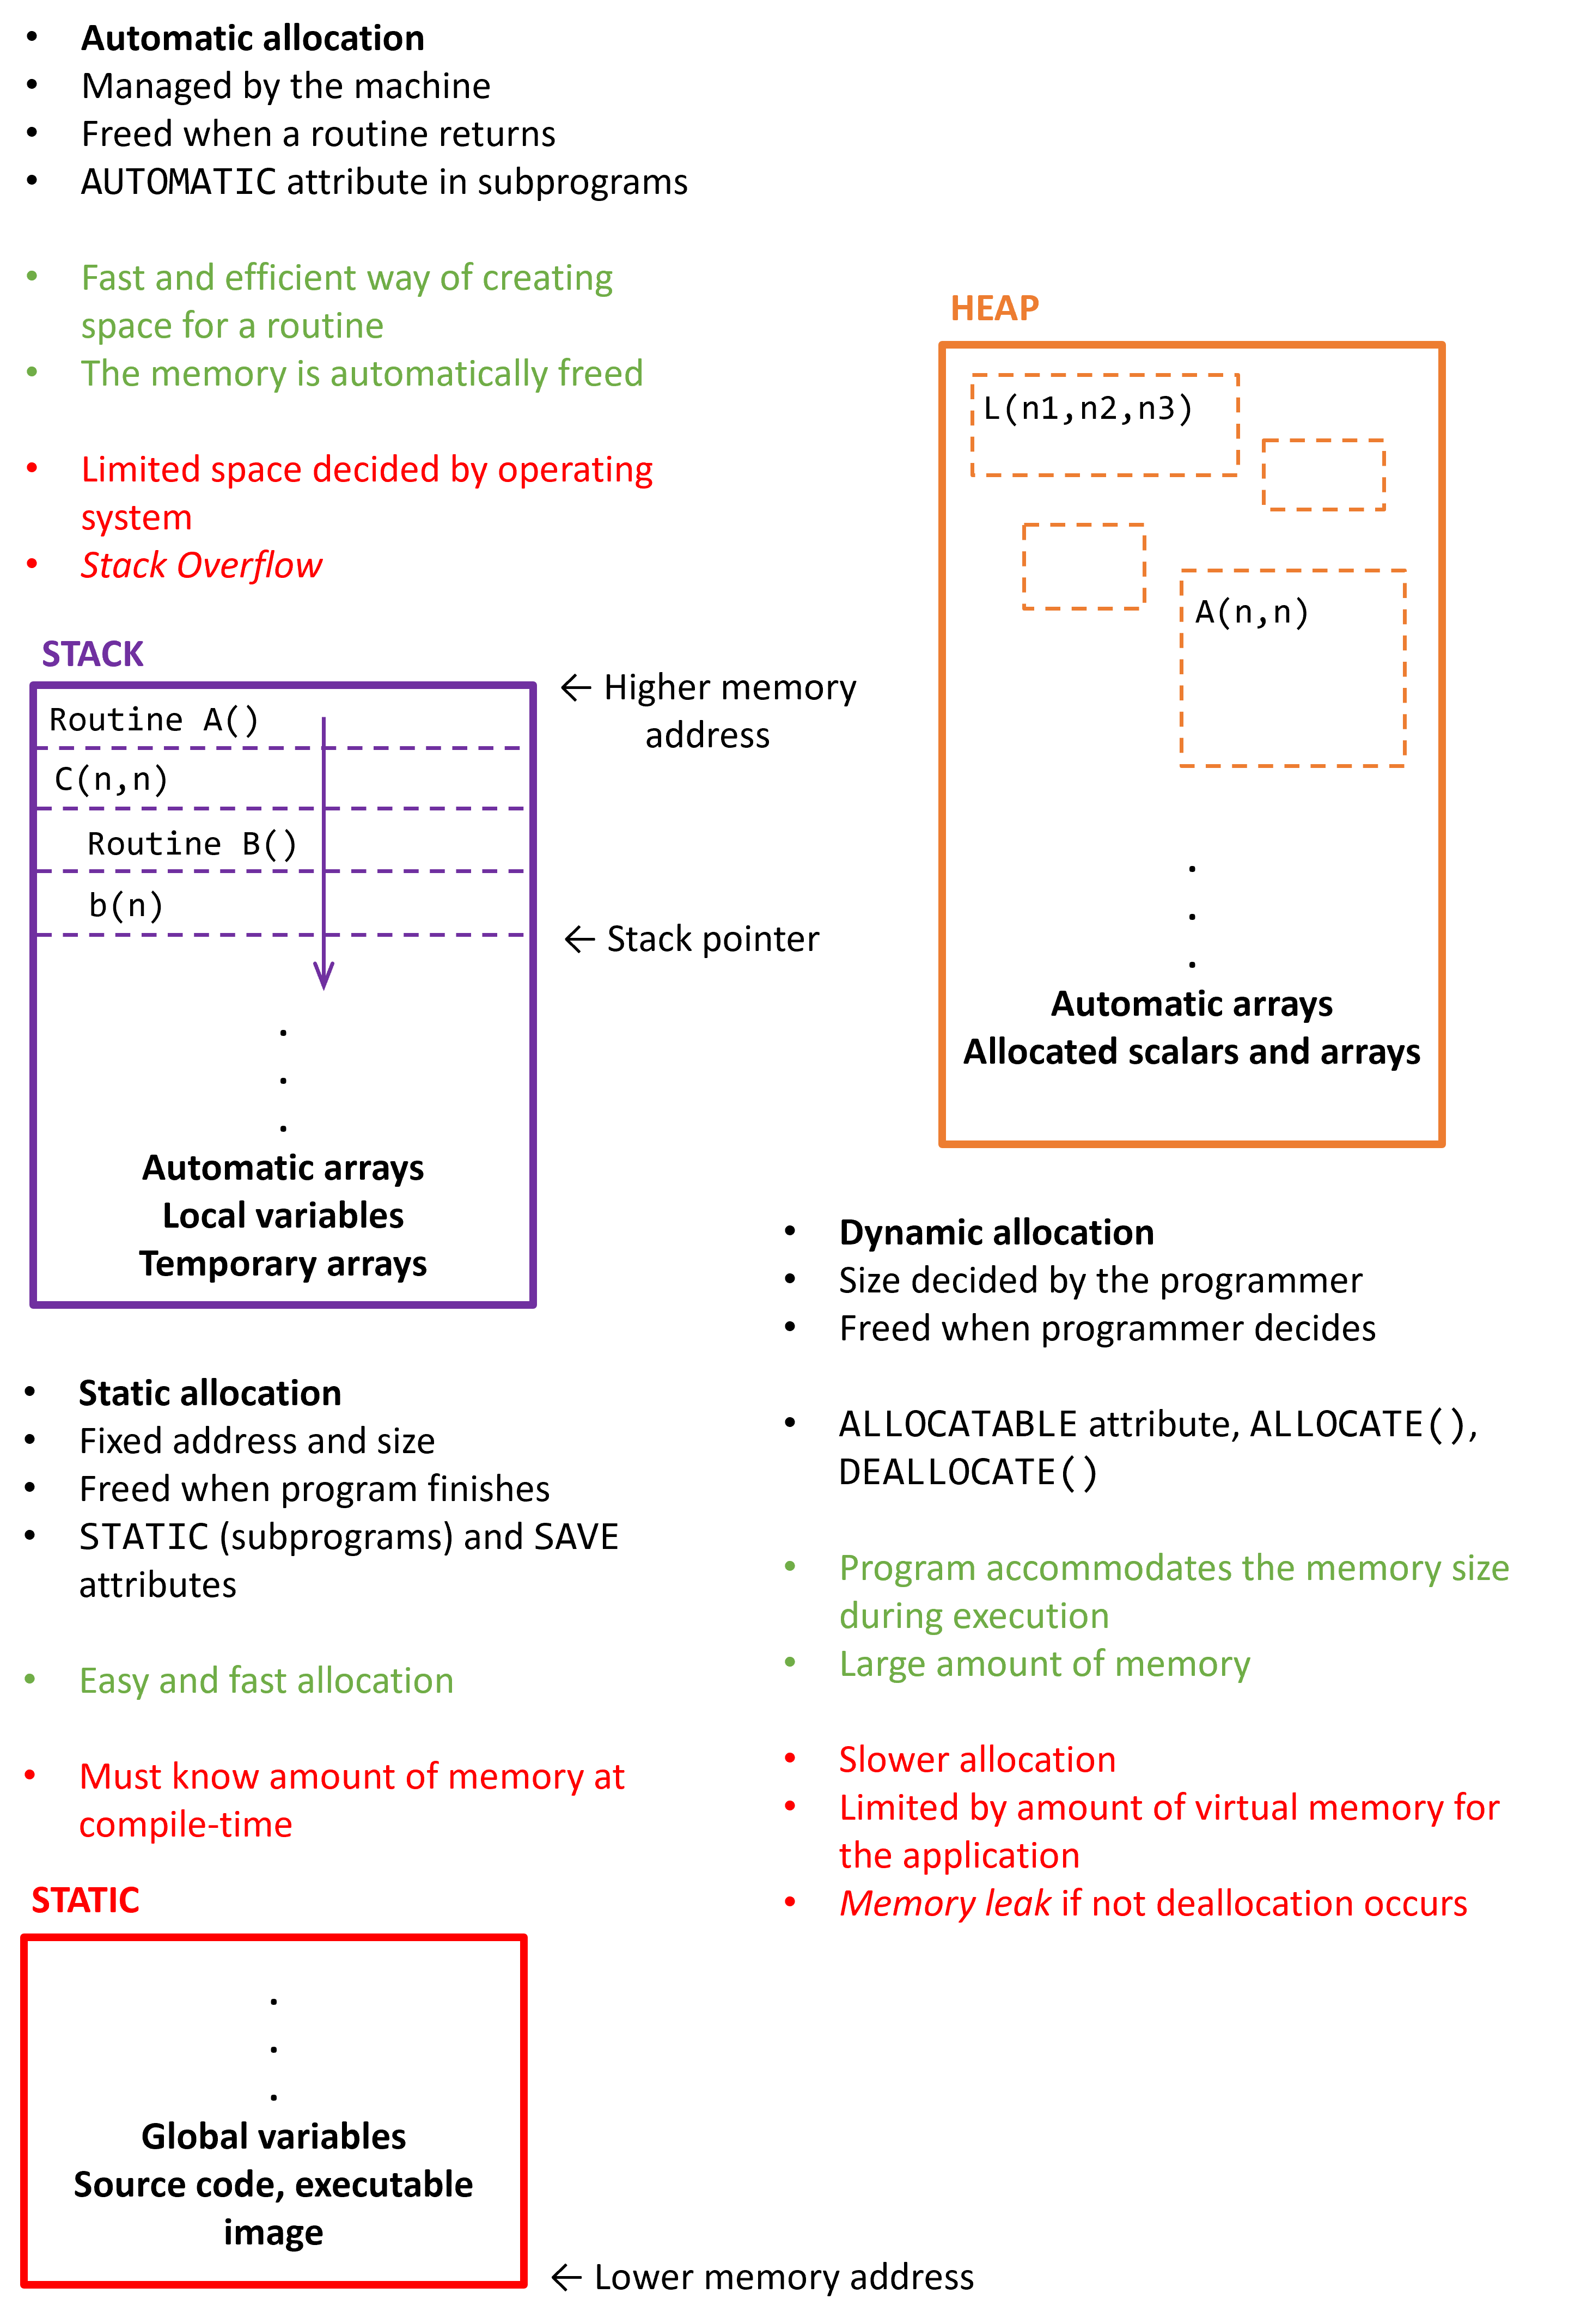
\includegraphics[width= \textwidth]{./doc/Figures/Memories.png}
    \caption{Three memory regions used by a program and the advantages and disadvantages associated to their allocation.}
    \label{fig:Memories}
\end{figure}






%-------------------------------------------------------------------------------------------------------------
%MAYBE INTERESTING IN FUTURE:

%When using AUTOMATIC, SAVE, STATIC, etc.
%\item How to manage it in your program and recommendations.
%\item How to reserve more space in each of them.


%-------------------------------------------------------------------------------------------------------------
%Revise the following concepts:
%
%\begin{enumerate}
%    \item Who manages the memory.
%    \item Where are physically stored (RAM, swap).
%    \item Which is faster to allocate and use.
%    \item Common problems related to the use of that memory.
%    \item How to manage it in your program and recommendations.
%    \item How to reserve more space in each of them.
%    \item etc.
%\end{enumerate}


%  Fortran for example uses this memory to create space for local arrays (those based on arguments of routines) or for temporary copies in array expressions. 
%     the stack is managed by the CPU, there is no ability to modify it
% variables are allocated and freed automatically

%  under the \texttt{deallocate} statement (in the case of Fortran)
  